\chapter{Konzeption}

\section{Bewertungskriterien}
 
\section{Bewertung vorhandener Lösungalternativen}

Im Folgenden werden die 3 Alternativen nacheinander mit Hilfe der oben genannten Heuristiken/Kriterien bewertet, und abschließend ein vergleichendes Fazit in Form einer Tabelle \todo{ref auf tabelle?} gezogen.

\section{Bewertung der Lösungsalternativen}

\todo{Punkte auf Konsistenz überprüfen}
\begin{sidewaystable}[ht]
	\centering
	\caption{Vergleich der Lösungsalternativen}
	\vspace*{10px}
	\label{tab:nielsen}
	\begin{tabular}{r|l|c|c|c|}
	\cline{2-5}
    	        				    &								& Photo Measures 	& Measuring Master 	& Measure \& Sketch \\ \cline{2-5} 
	Nach \cite{Nielsen94} 	& \autoref{itm:1}				&       \po 		&    \po 			&       \xmark      \\ \cline{2-5} 
    	             				& \autoref{itm:2} 				&       \po  		&    \po  			&       \po		    \\ \cline{2-5}
    	             				& \autoref{itm:3} 				&       \xmark 		&    \po			&       \xmark      \\ \cline{2-5} 
    	             				& \autoref{itm:4} 				&       \po  		&    \po			&       \xmark      \\ \cline{2-5}
    	            				& \autoref{itm:5} 				&       \po  		&    \xmark			&       \xmark      \\ \cline{2-5} 
    	            				& \autoref{itm:6} 				&       \xmark 		&    \po  			&       \xmark      \\ \cline{2-5} 
    	             				& \autoref{itm:7} 				&       \po  		&    \xmark			&       \xmark      \\ \cline{2-5} 
    	             				& \autoref{itm:8} 				&       \nl  		&    \po  			&       \xmark      \\ \cline{2-5} 
    	             				& \autoref{itm:9} 				&       \po   		&    \po  			&       \nl	        \\ \cline{2-5} 
    	            				& \autoref{itm:10} 				&       \po  		&    \po 			&       \xmark      \\ \cline{2-5} 
    	             				& \autoref{itm:11} 				&       \po   		&    \po 			&       \xmark      \\ \cline{2-5} 
    	             				& \autoref{itm:12} 				&       \po   		&    \po 			&       \xmark      \\ \cline{2-5} 
    	             				& \autoref{itm:13}			 	&       \xmark  	&    \xmark			&       \xmark      \\ \cline{2-5} 
    	            				& \autoref{itm:14} 				&       \po   		&    \po  			&       \po		    \\ \cline{2-5}
    	            				& \autoref{itm:15} 				&       \po   		&    \xmark			&       \xmark  	\\ \cline{2-5}   
    	            				& \autoref{itm:16} 				&       \po   		&    \po  			&       \xmark      \\ \cline{2-5} 
    	             				& \autoref{itm:17} 				&       \po  		&    \po  			&       \xmark		\\ \cline{2-5} 
    	             				& \autoref{itm:18} 				&       \nl  		&    \nl 			&       \nl		    \\ \cline{2-5} 
	Eigene Kriterien 				& \autoref{itm:integration}		&      	\xmark		&    \xmark			&       \xmark      \\ \cline{2-5}
	    	         				& \autoref{itm:export}   		&      	\xmark		&    \xmark			&       \xmark      \\ \cline{2-5}

	    	             
	\end{tabular}
	\\
	\vspace*{10px}
	\begin{tabular}{l}
		\po~wird erfüllt \\
		\nl~wurde nicht berücksichtigt \\
		\xmark~wird nicht erfüllt
	\end{tabular}
\end{sidewaystable}

\clearpage
\section{Vorgehensweise bei Implementierung eigener Software-Lösung}
\todo{Alle Aussagen mit Zitaten belegen?}
\todo{Schreiben was ich in dieser section mache}
\todo{Bezug auf Ergebnisse von alternativen} 
 \subsection{Die 8 Goldenen Regeln von Shneiderman}
 
\citeauthor{Shneiderman04} definieren in ihrem Buch ``Designing the User Interface: Strategies for Effective Human-Computer Interaction'' die sogenannten ``8 Goldenen Regeln des Interface Designs''.  Die acht Regeln lauten wie folgt:

\begin{enumerate}
	\item Bemühe Dich um Konsistenz (``Strive for consistency'')
	\item Erlaube erfahrenen Benutzern die Nutzung von Abkürzungen (``Enable fequent users to use shortcuts'')
	\item Biete informative Rückkopplung (``Offer informative feedback'')
	\item Biete ein klares Ende von Teildialogen an (``Design dialogs to yield closure'')
	\item Biete Fehlervermeidung und einfache Fehlerbehandlung an (``Offer error protection and simple error handling'')
  \item \label{itm:undo} Erlaube eine einfach Rücknahme von Aktionen (``Permit easy reversal of actions'')
	\item Gib dem Benutzer die Kontrolle (``Support internal locus of control'')
	\item Minimiere Gedächtnisbelastung (``Reduce short-memory load'')
\end{enumerate} 

Diese Regeln sind ein weiterer guter Anhaltspunkt für die Entwicklung einer guten Software-Lösung, die den Faktor der Usability mit berücksichtigt. Vor allem der Punkt \autoref{itm:undo} sollte bei einer Applikation, deren Fokus auf den aneinander gereihten Aktionen des Benutzers beruht, erfüllt sein. Dies soll durch einen Undo- bzw. Redo-Button in der oberen Menüleiste gewährleistet werden. \\

Die Konsistenz der Applikation soll durch die Benutzung der \citet{AndroidMG} gewährleistet werden. 
So werden einerseits nur Icons aus der Standard Google-Library verwendet, andererseits werden diverese Guidelines die auf \citet{AndroidMG} vorgestellt werden, benutzt. 
Hierzu zählt auch die sogenannte \emph{Feature-Discovery}.
Dabei soll der Benutzer durch ein hinweisendes Overlay dazu aufgefordert werden, gewisse Funktionen der App zu erkunden. 
Dies ist besonders bei einer App, in der es mehr als eine zentrale Funktion gibt, hilfreich und wichtig. \\

\begin{figure}[h]
    \centering
    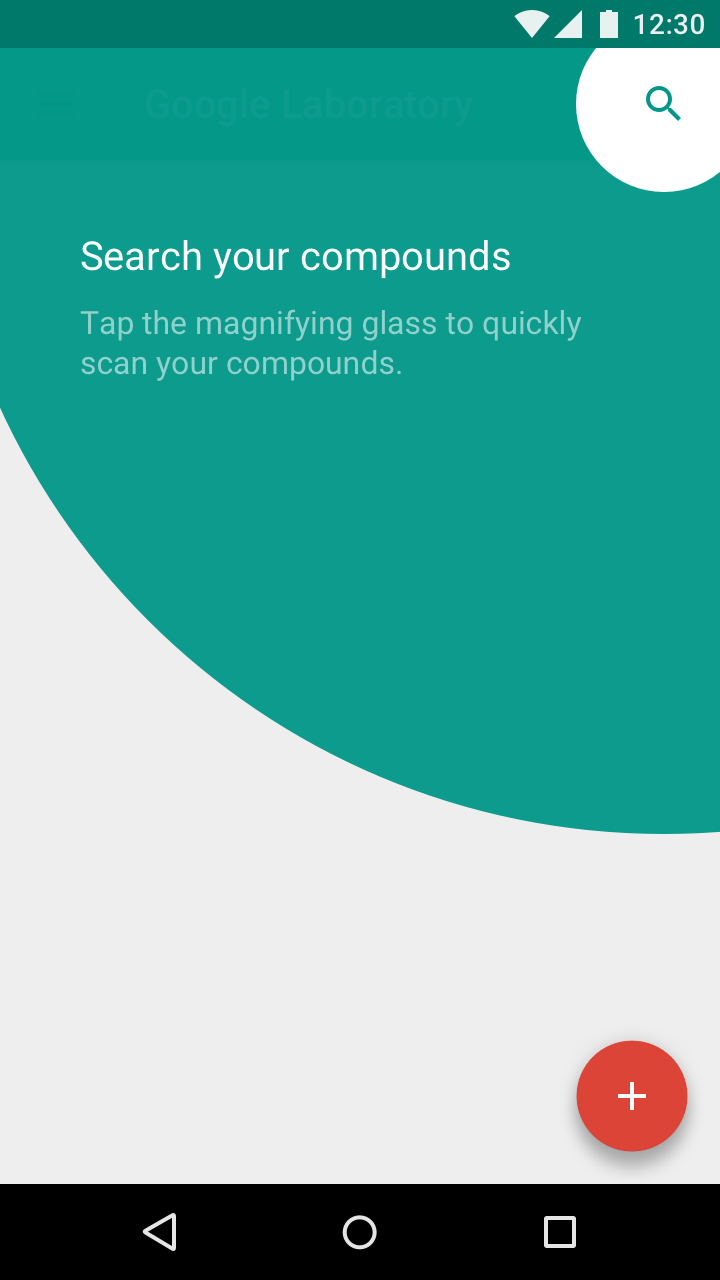
\includegraphics[keepaspectratio, width=0.5\textwidth]{fd}
    \caption{Feature-Discovery in Form eines Tap-Targets}
    \label{fig:fd}
\end{figure}

In \autoref{fig:fd} sieht man eine beispielhafte Implementierung einer solchen Feature-Discovery in Form eines Tap-Targets.
Hierbei wird der Benutzer durch eine Hervorhebung bestimmter UI-Elemente auf Funktionen hingewiesen. 
Zusätzlich wird ein kurzer erklärender Satz mit einem zusammenfassenden Titel angezeigt. \\

\subsection{Gesture-Support}

Mit der Einführung Applikationen für mobile Endgeräte hat sich ein weiteres, vorher nicht relevantes, Usability-Problem etabliert: 
\emph{Die geringe Größe des Bildschirm}. \\

Die relativ kleine physikalische Größe der Smartphone-Displays bringt verschiedene Probleme mit sich. 
So muss einerseits die Funktionalität einer ganzen Desktop-Applikation auf ein viel kleineres Display passen, ohne den Content zu verändern, oder gar unleserlich zu machen.
Andererseits muss dem Benutzer eine intuitive und effiziente Navigationsmöglichkeit gegeben sein, um zwischen verschiedenen Inhalten zu wechseln. \\

Hierzu schreiben \citeauthor{Gutwin04}, dass die Navigationen auf kleinen Bildschirmen selbst im besten Fall deutlich langsamer sei als auf normal-großen Bildschirmen.
Sie führen weiter an, dass eine Übersicht über den gesamten Systemzustand wertvoll sei, da dies dem Nutzer eine schnellere Navigation erlaube. \\
Nach \citeauthor{Gutwin04} eigne sich die Technik des ``Two-Level Zooms'' besonders gut für Navigationsaufgaben, wohingegen Panning-Strategien eher negativ von den Test-Personen aufgenommen worden seien \citep[Seite 8]{Gutwin04}.  

\todo{Tap-Target prompts}

\subsection{Iterativer Entwicklungsprozess}
  3 Iterationen jeweils Mitte Dezember, Januar und Februar \\
  Feedback in Form von Gitlab-Issues und Beobachten von Testpersonen (Usability-Experimente) \\
  1. Iteration (Dezember): App mit floating buttons (screenshots vorher-nachher)
  2. Iteration (Januar): App mit status bar (screenshots vorher-nachher)
  3. Iteration (Februar): App mit Help-Overlay \& verbesserter Statusbar (screenshots vorher-nachher)
\subsection{DIN und ISO-Normen}
\subsection{Material Design-Guidelines}
\subsection{ABC-Modell}
\subsection{Gesture-Support (papers)}
  Zoom-Area und Panning am besten geeignet um Content auf kleinen Displays darzustellen \\
  
